%\documentclass[11pt]{article}
%\usepackage{beamerarticle}
%\usepackage{graphicx}
\documentclass[12pt,xcolor=dvipsnames,handout
   ]{beamer}
%\PassOptionsToClass{beamer}{handout}
% \usepackage{pgfpages} 
% \pgfpagesuselayout{4 on 1}[letterpaper,landscape,border shrink=3mm]
\usepackage{amsmath}
\usepackage{helvet}
\usepackage{mymacros}
\usepackage{xspace}
\usepackage[all,cmtip,arrow]{xy}  %for xy-pic fonts
%%macs
\newcommand{\V}{\ensuremath{\mathcal V}\xspace}
\newcommand{\mbold}[1]{\ensuremath{\mathbf{#1}}\xspace}
\makecs{\mbold}{ABDP}
\newcommand{\exmpl}[1]{{\color{green!50!black} #1}}
\newcommand{\dsize}{\displaystyle}
\DeclareMathOperator{\End}{End}
\DeclareMathOperator{\Var}{Var}
\DeclareMathOperator{\Cg}{Cg}
\DeclareMathOperator{\Sub}{Sub}
\DeclareMathOperator{\Con}{Con}
\DeclareMathOperator{\Rel}{Rel}
\newcommand{\bigpause}{\pause\bigskip}
\DeclareMathOperator{\CSP}{CSP}
\newcommand{\FF}{\mathbb{F}}
\DeclareMathOperator{\Pol}{Pol}
\DeclareMathOperator{\Inv}{Inv}
\renewcommand{\.}{\cdot}
\DeclareMathOperator{\core}{core}
\newcommand{\reduc}{\leq_{\text{\textnormal{p}}}}
\newcommand{\equivp}{\equiv_{\text{\textnormal{p}}}}
\newcommand{\NP}{\ensuremath{\mathbb{NP}}\xspace}
\renewcommand{\P}{\ensuremath{\mathbb{P}}\xspace}
\newcommand{\Blue}{\textcolor{blue!50!black}}
\newcommand{\Red}{\textcolor{violet!50!red}}
\newcommand{\Green}{\textcolor{green!55!black}}
\let\origemph=\emph 
\let\origtextbf=\textbf 
%%endmacs
%%
\parskip=10pt
%% Beamer Setup
\mode<handout>{\beamertemplatesolidbackgroundcolor{black!5}}
\mode<presentation>{
  \usetheme{Singapore}
  \usetheme{Frankfurt}
%  \useinnertheme[shadow]{rounded}
  \setbeamertemplate{navigation symbols}[only frame symbol]{}
}
\mode<beamer>
{%
  \let\emph=\alert
  \renewcommand{\textbf}[1]{{\usebeamercolor[fg]{example text}%
     \origtextbf{#1}}}
}
\mode<article>{\usepackage{fullpage}}
%%
%\title{\TeX\ and \LaTeX\ in the Mathematics Department}
%\author{Clifford Bergman}

\begin{document}
\title{Constraint Satisfaction Problems,\\Graph Theory,\\and Universal Algebra}
\frame[plain]{\titlepage}

\begin{frame}
\frametitle{What is a CSP?}

  Informally, a \textbf{C}onstraint \textbf Satisfaction \textbf Problem
  consists of
  \begin{itemize}
  \item a list of variables ranging over a finite domain and
  \item a set of constraints on those variables.
  \end{itemize}

  \textbf{Problem:} can we assign values to all the variables so that
  all of the constraints are satisfied?

\end{frame}

\begin{frame}
  \frametitle{Examples}

A system of linear equations is a CSP
\begin{alignat*}4
  a_{11}x_1 &&+ a_{12}x_2 &&+ \cdots &&+ a_{1n}x_n &= b_1 \\
  a_{21}x_1 &&+ a_{22}x_2 &&+ \cdots &&+ a_{2n}x_n &= b_2 \\
  &&\;\vdots \\
  a_{m1}x_1 &&+ a_{m2}x_2 &&+ \cdots &&+ a_{mn}x_n &= b_m \\
\end{alignat*}
\end{frame}

\begin{frame}
  Also, a system of nonlinear equations is a CSP
\begin{alignat*}4
  a_{11}x_1^2x_3 &+ a_{12}x_2x_3x_7 &&+ \cdots &&+ a_{1n}x_4x_n^3 &&= b_1 \\
  a_{21}x_2x_5 &+ a_{22}x_2 &&+ \cdots &&+ a_{2n}x_4^3 &&= b_2 \\
 &&\;\vdots \\
  a_{m1}x_3x_5x_8 &+ a_{m2}x_2 &&+ \cdots &&+ a_{mn}x_n &&= b_m \\
\end{alignat*}
\end{frame}

\begin{frame}
  For a fixed $k$, determining whether a graph is $k$-colorable is a CSP
  \begin{center}
    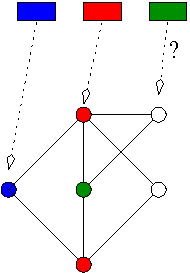
\includegraphics{k-col}
%    \fbox{picture suggesting 3-colorability}
  \end{center}
\end{frame}

\begin{frame}
  \frametitle{Algorithms}
  There is an efficient algorithm (Gaussian elimination) for solving any
  linear system.
  That is

\setbeamercolor{block body example}%
{parent=normal text,use=block title example,bg=block title example.bg!25!bg}
  \begin{exampleblock}{}
    There is an algorithm that accepts as \textbf{input} a linear system
    and decides whether that system has a solution.

    \smallskip
    The running time of the algorithm is bounded above by $f(s)$ where
    $f$ is a polynomial and $s$ is the size of the system.
  \end{exampleblock}
  \pause

  The particular system is an \textbf{instance} of the \textbf{problem}
  LINEAR SYSTEM
  
\end{frame}

\begin{frame}
  Similarly

  \setbeamercolor{block body example}%
  {parent=normal text,use=block title example,bg=block title example.bg!25!bg}
  \begin{exampleblock}{}
    There is an algorithm that accepts as input a graph and decides
    whether the graph is 2-colorable.

    \smallskip
    The running time is bounded by $f(s)$ where $f$ is a polynomial and
    $s$ is the size of the graph.
  \end{exampleblock}

  The graph is an instance of the problem 2-COLORABILITY.

  \pause
  We say these algorithms run in \emph{polynomial time}.
\end{frame}

\begin{frame}
  No polynomial-time algorithm is known for either NONLINEAR SYSTEM or
  3-COLORABILITY. 

  \bigpause
  However, any candidate solution to either of these problems can be
  checked in polynomial-time. 

  \bigpause
  Thus these problems are solvable in \emph{nondeterministic polynomial
    time.} 
\end{frame}

\begin{frame}
  Let $X$ and $Y$ be two problems. We write $X \reduc Y$ to indicate that
  $Y$ is at least as hard as $X$.

  \bigpause
  Somewhat more precisely: any algorithm for solving $Y$ can be
  transformed into an algorithm for $X$ without drastically increasing
  its running time.

  \bigpause
  It is possible for $X\reduc Y \reduc X$. In that case, write $X\equivp
  Y$. 

\end{frame}

\begin{frame}
  \P is the class of all problems solvable in polynomial time. Its
  members are called \emph{tractable.}

  \NP is the class of problems solvable in nondeterministic polynomial
  time. 

  \pause
  \begin{itemize}
  \item $\P \sseq \NP$
  \item Both $\P$ and $\NP$ are downsets, i.e., \\
    $Y\in \P \mathrel{\&} X\reduc Y \implies X\in \P$
  \end{itemize}

  \pause
  The maximal members of \NP are called \emph{\NP-complete.} 

  
  Both 3-COLORABILITY and NONLINEAR SYSTEM are known to be
  \NP-complete. 
\end{frame}

\begin{frame}
  \frametitle{\$$2^{20}$ question: $\P \overset{?}{=} \NP$.}

  \pause
  If $\P=\NP$ then all of the above distinctions go away. Almost every
  problem that mathematicians actually care about can be solved
  efficiently. Just build bigger computers.

  \pause
  In particular, this talk becomes pointless. So assume $\P\neq \NP$.

  \pause
  \begin{theorem}[Ladner, 1975 \cite{Ladner1975}]
    If $\P \neq \NP$ then there are problems in $\NP-
    \P$ that are not \NP-complete.
  \end{theorem}

\end{frame}

\begin{frame}
  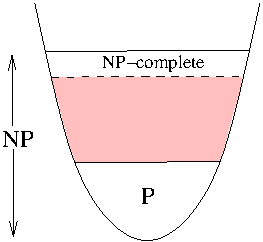
\includegraphics[scale=1.25]{complexity}
  \qquad
  \parbox[b][2in][c]{1.5in}{If $\P\neq \NP$ then the pink area is nonempty.}
\end{frame}

\begin{frame}
  \frametitle{Formal Definition of CSP}

  Let $D$ be a set, $n$ a positive integer\\
  An \emph{$n$-ary relation on $D$} is a subset of $D^n$

  \pause
  $\Rel_n(D)$ denotes the set of all $n$-ary relations on $D$

  $\Rel(D) = \bigcup\limits_{n>0} \Rel_n(D)$
\end{frame}

\begin{frame}
  Let $D$ be a finite set and $\Delta\sseq \Rel(D)$

  $\CSP(\<D,\Delta\>)$ is the problem:\\
  \textbf{instance:} A finite set $V=\setof{v_1,\dots,v_n}$ of
    \emph{variables}
    and\\
    a finite set $\setof{C_1,\dots,C_m}$ of \emph{constraints}

    Each constraint $C_i$ is a pair $(\seqof{x_{i1},\dots,x_{i\,p_i}},\,
    \delta_i)$ in which $x_{i1},\dots,x_{i\,p_i} \in V$ and $\delta_i\in
    \Delta$

    \pause
    \textbf{Question:} Does there exist a mapping $f\colon V\to D$ such
    that for all $i\leq m$, $\<f(x_{i1}),\dots,f(x_{i\,p})\>\in \delta_i$?

    \pause
    $\CSP(\<D,\Delta\>)$ always lies in \NP.

    $\CSP\<D,\Delta\>$ is \emph{finitary} if $\Delta$ is finite. 
\end{frame}

\begin{frame}
  \frametitle{Example: Linear Equations over $\FF_2$}

  $D=\{0,1\}$ \\
  $\Delta$ consists of all relations
  \begin{equation*}
    \delta_{n,\mathbf a}^b = \bigl\{\,\<x_1,\dots,x_n\>\in D^n :
      a_1x_1+\cdots a_nx_n = b\bigr\}
  \end{equation*}

  Then $\CSP(\<D,\Delta\>)$ is the linear equations problem
\end{frame}

\begin{frame}
  \frametitle{Example: 3-colorability}

  $D=\{\Red{r},\Green{g},\Blue{b}\}$, $\Delta=\{\kappa_3\}$\\
  $\kappa_3=\setof{(x,y)\in D : x\neq y}$

  Then $\CSP(\<D,\Delta\>)$ is the 3-colorability problem

  \bigskip

    \begin{columns}
      \begin{column}{1.5in}
        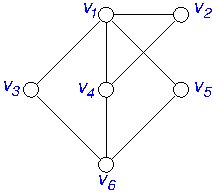
\includegraphics{col_csp}
      \end{column}
      \begin{column}{2in}
        $V=\{v_1,\dots,v_6\}$\\
        $\<v_1,v_2\>\in \kappa$\\
        $\<v_1,v_3\>\in \kappa$\\
        $\<v_1,v_4\>\in \kappa$\\
        $\<v_2,v_4\>\in \kappa$\\
        \qquad$\vdots$\\
        $\<v_5,v_6\>\in \kappa$
      \end{column}
    \end{columns}
  \end{frame}

\begin{frame}
  \frametitle{Schaefer's Dichotomy}

  \begin{theorem}[Schaefer, 1978 \cite{Schaefer1978}]
    Let $D=\{0,1\}$. There are six families $\Delta_1,
  \dots, \Delta_6$ such that
  \begin{equation*}
    \CSP(\<D,\Delta\>) \in \P \iff \Delta \sseq \Delta_i, \text{some $i\leq 6$}
  \end{equation*}
  Otherwise $\CSP(\<D,\Delta\>)$ is $\NP$-complete.
\end{theorem}
\end{frame}

\begin{frame}
  \frametitle{Two Motivating Questions}

  \begin{enumerate}
  \item \emph{Dichotomy Conjecture}\\ Every $\CSP(\<D,\Delta\>)$ either
    lies in \P\ or is $\NP$-complete.

    \pause

  \item \emph{Tractability Problem}\\ Characterize those CSPs that lie in \P.
  \end{enumerate}
\end{frame}

\begin{frame}
  \frametitle{Graph Homomorphisms}

  Well-known fact: A graph $G$ is 3-colorable iff there is a
  graph homomorphism from $G$ to $K_3$. 

  \pause

  \begin{definition}
    Let $\<G,E\>$ and $\<H,F\>$ be (di)graphs. A \emph{homomorphism} is
    a function $f\colon G \to H$ such that $$(x,y)\in E \implies
    \bigl(f(x),\, f(y)\bigr) \in F.$$
  \end{definition}

  \pause

  \textbf{Remark.} This definition makes sense
  \begin{itemize}
  \item  for both undirected and directed graphs;
  \item for graphs with all/some/no loops.
  \end{itemize}

\end{frame}

\begin{frame}
  \begin{center}
    3-Coloring $G$ as a homomorphism to $K_3$

    \includegraphics{3col}
  \end{center}
\end{frame}

\begin{frame}
  \begin{definition}
    Let $H$ be a digraph. $\CSP(H)$ is the problem:\\
    \emph{Instance:} A digraph $G$\\
    \emph{Question:} Is there a homomorphism from $G$ to $H$?
  \end{definition}

  Note that $\CSP(H)$ is a constraint satisfaction problem. (The
  ``$H$-coloring'' problem.)

  \pause
  \begin{theorem}[Feder and Vardi, 1998 \cite{FederVardi1998}]
    For every finitary CSP $X$ there is a digraph $H$ such that
    $X\equivp \CSP(H).$
  \end{theorem}

\end{frame}

\note{So if you want to solve the dichotomy problem, it is enough to
  look at graphs.}

\begin{frame}
  \frametitle{The CSP for Graphs}

  \begin{definition}
    Let $H$ be a digraph.
    \begin{enumerate}
    \item An induced subgraph $H'$ is a \emph{retract} of $H$ if there
      is $r\colon H \to H'$ with $r\circ r = r$.
    \item A \emph{core} of $H$ is a minimal retract.
    \end{enumerate}
  \end{definition}

  \pause
  Easy fact: any two cores of $H$ are isomorphic. 

  $H$ is called a \emph{core} if $H=\core(H)$. 
\end{frame}

\begin{frame}
  \begin{lemma}
    For any digraph $H$, $\CSP(H)\equivp \CSP(\core(H))$.
  \end{lemma}

  \pause

  \begin{theorem}[Hell \& Ne\v set\v ril, 1990 \cite{HellNesetril1990}]
    Let $H$ be an undirected, loopless graph. Then $\CSP(H)$ lies in
    \P\ if and only if $H$ is bipartite, otherwise it is \NP-complete. 
  \end{theorem}

  \pause
  
  \begin{corollary}
    The dichotomy conjecture holds for undirected graphs.
  \end{corollary}
\end{frame}

\begin{frame}
  \begin{theorem}[Barto, Kozik and Niven, 2008 \cite{BartoKozikNiven2008}]
    Let $H$ be a smooth digraph. If each component of $\core(H)$ is a
    circle, then $\CSP(H)\in \P$. Otherwise $\CSP(H)$ is \NP-complete.    
  \end{theorem}

  \pause
  $H$ is \emph{smooth} if each vertex has an incoming and an outgoing
  edge. 

  A \emph{circle} is a directed cycle with no chords.

  \begin{corollary}
    The dichotomy conjecture holds for smooth digraphs.
  \end{corollary}
\end{frame}


\begin{frame}
  \frametitle{Polymorphisms}

  \begin{definition}
    Let $\delta \in \Rel_k(D)$ and $f\: D^n \to D$. We say 
    \emph{$f$ preserves $\delta$} if
    \begin{equation*}
      \begin{split}
        (a_{11}, \dots, a_{1k}),&\dots, (a_{n1},\dots, a_{nk}) \in
        \delta \implies\\ 
        &\bigl( f(a_{11},\dots, a_{n1}), \dots, f(a_{1k},\dots,a_{nk})
        \bigr) \in \delta
    \end{split}
    \end{equation*}

  \end{definition}

  \begin{overprint}
  \onslide<2|handout:0>
  $f$ is an \emph{$n$-ary operation} on $D$.
  % 
  \onslide<3|handout:1>
    \begin{equation*}
      \newcommand\flab{\scriptstyle{f}}
      \begin{matrix} a_{11} & a_{12} & \dots & a_{1k} & \in & \delta \\
        a_{21} & a_{22} & \dots & a_{2k} & \in & \delta \\
        \vdots  & \vdots &       &\vdots  &     & \vdots \\
        a_{n1} & a_{n2} & \dots & a_{nk} & \in & \delta \\
        \downarrow\flab &\downarrow\flab &  & \downarrow\flab \\
        \star  & \star  & \dots & \star  & \in & \delta
      \end{matrix}
    \end{equation*}
  \end{overprint}
\end{frame}

\begin{frame}
  \begin{definition}
    Let $\Delta$ be a set of relations on $D$. Then
    \emph{$\Pol(\Delta)$} denotes the set of all operations preserving
    all members of $\Delta$. These are the \emph{polymorphisms} of
    $\Delta$. 

    \bigpause

    Let $F$ be a set of operations on $D$. Then \emph{$\Inv(F)$} denotes
    the set of all relations preserved by all operations in $F$.
  \end{definition}
\end{frame}

\begin{frame}
  \begin{theorem}
    Let $\Gamma, \Delta \sseq \Rel(D)$. Then
    \begin{equation*}
      \Pol(\Gamma) \sseq \Pol(\Delta) \implies \CSP(\Delta) \reduc
      \CSP(\Gamma). 
    \end{equation*}
  \end{theorem}

\pause
Note: $\Delta$ is a core iff $\Pol_1(\Delta)$ is a set of permutations of $D$.\\
$\Pol_1(\Delta)$ is the set of unary polymorphisms

\end{frame}

\begin{frame}
  One can go back and forth between relational and algebraic structures

  \begin{center}
    \begin{tabular}{ccc}
      \origtextbf{Relational} & &\origtextbf{Algebraic}  \\
      $\<D,\Delta\>$ & $\longrightarrow$ & $\<D,\Pol(\Delta)\>$ \\[2pt]
      $\<D, \Inv(F)\>$ & $\longleftarrow$ &$\<D,F\>$
    \end{tabular}
  \end{center}

  $\CSP\<D,\Delta\> \equivp \CSP\<D,\Inv(\Pol(\Delta))\>$

  \bigpause
  Perhaps the expressive power of algebra can be used to classify CSPs.

  Notation: $\CSP(F) = \CSP(\Inv(F))$
\end{frame}

\begin{frame}
  \frametitle{Algebraic Facts}

  Let \A\ and \B\ be algebras

  $\B \text{ a subalgebra of \A} \implies \CSP(\B) \reduc \CSP(\A)$.

  $\B \text{ a homomorphic image of \A}\implies \CSP(\B) \reduc
  \CSP(\A)$. 

\end{frame}

\begin{frame}
Let $\Delta \sseq \Rel(D)$. \\
For $a\in D$ write $\mu_a=\{a\} \in \Rel_1(D)$\\
$\Delta^* = \Delta \cup \setof{\mu_a : a\in D}$.

Every member of $\Pol(\Delta^*)$ is \emph{idempotent,} that is,
$f(x,x,\dots,x)=x$. 

\bigpause

\begin{theorem}[Bulatov, Jeavons, Krokhin, 2000
  \cite{BulatovKrokhinJeavons2000}] 
  If $\Delta$ is a  core then $\CSP(\Delta) \equivp \CSP(\Delta^*)$.
\end{theorem}

\begin{corollary}
  For every algebra \A, there is an idempotent algebra \B\ such that
  $\CSP(\A) \equivp \CSP(\B)$.
\end{corollary}
\end{frame}

\begin{frame}
  \begin{corollary}
    For every algebra \A, there is an idempotent algebra \B\ such that
    $\CSP(\A) \equivp \CSP(\B)$.
  \end{corollary}

  \B\ is efficiently computable from \A.
  
  Thus for our two questions, we can restrict our attention to idempotent
  algebras.

\end{frame}

\begin{frame}
  \frametitle{CSP results for Algebras}

  \begin{theorem}[Jeavons, Cohen, Gyssens, 1997
    \cite{JeavonsCohenGyssens1997}]
    If $\Pol(\Delta)$ contains a semilattice operation, then
    $\CSP(\Delta) \in \P$. 
  \end{theorem}

  semilattice: $x\.(y\.z) = (x\.y)\.z,\quad x\.y = y\.x, \quad x\.x = x$

  \pause
  Examples: logical `$\meet$', `$\join$'; `$\cap$', `$\cup$', `$\gcd$',
  `$\operatorname{lcm}$', $\<H,K\>\in \Sub(G)$,\dots

\end{frame}

\begin{frame}
  \begin{theorem}[Bulatov, 2002 \cite{BulatovDalmau2006}]
    If $\Pol(\Delta)$ contains a Maltsev operation, then
    $\CSP(\Delta)\in \P$.
  \end{theorem}

  Maltsev: $q(x,x,y)= q(y,x,x) = y$

  Examples: groups, quasigroups, Boolean algebras, etc.

  \bigpause
  \begin{corollary}
    Both 2-COLORABILITY and LINEAR SYSTEM  are tractable.
  \end{corollary}

\end{frame}

\begin{frame}
  \begin{theorem}[Jeavons, Cohen, Gyssens, 1997 (?)
  \cite{JeavonsCohenGyssens1997}]
    If $\Pol(\Delta)$ contains a majority operation, then $\CSP(\Delta)
    \in \P$. 
  \end{theorem}

  majority: $m(x,y,y) = m (y,x,y) = m(y,y,x) = y$

  This gives another proof that 2-COLORABILITY is tractable
\end{frame}

\begin{frame}
  \begin{theorem}[Bulatov, Jeavons, Krokhin, 2000
    \cite{BulatovKrokhinJeavons2000}]
    If $\Delta$ is a core and every polymorphism is essentially unary,
    then $\CSP(\Delta)$ is \NP-complete.
  \end{theorem}

  $f$ is \emph{essentially unary} if $f(x_1,\dots,x_n) = g(x_j)$ for
  some unary $g$ and some $j\leq n$.

 \pause
 \begin{corollary}
    Both 3-COLORABILITY and NONLINEAR SYSTEM are \NP-complete.
  \end{corollary}
\end{frame}

\begin{frame}
  \begin{center}
    \includegraphics{examples}
  \end{center}


  \textbf{Informal reformulation of the dichotomy conjecture}\\
  If \A\ has some
  kind of decent algebraic structure then $\CSP(\A) \in \P$ otherwise
  $\CSP(\A)$ is \NP-complete.
\end{frame}

% \begin{frame}
%   \begin{definition}
%     Let $n>1$. An $n$-ary operation $f$ is called a \emph{Taylor operation}
%     if it is idempotent and satisfies identities
%     \begin{align*}
%       f(x_{11}, x_{12}, \dots, x_{1n}) &= 
%       f(y_{11}, y_{12},\dots, y_{1n}) \\
%       f(x_{21}, x_{22}, \dots, x_{2n}) &= 
%       f(y_{21}, y_{22},\dots, y_{2n}) \\
%       &\vdots\\
%       f(x_{n1}, x_{n2}, \dots, x_{nn}) &= 
%       f(y_{n1}, y_{n2},\dots, y_{nn}) 
%     \end{align*}
%     in which every $x_{ij}$ and $y_{ij}$ is a variable and $x_{ii}\neq
%     y_{ii}$ for $i=1,\dots,n$. 
%   \end{definition}

%   \pause
%   Note that an essentially unary operation (on a nontrivial set) can not
%   be a Taylor operation. 
% \end{frame}

\begin{frame}
  \begin{definition}
    Let $n>1$. An $n$-ary operation $f$ is called a \emph{weak
      near-unanimity operation} if \\
    \hspace*{1em} it is idempotent\\
    and satisfies
    \begin{multline*}
    f(y,x,x,x,\dots,x) = f(x,y,x,x,\dots,x) = \cdots\\
    = f(x,x,\dots,x,y)
  \end{multline*}
  \end{definition}

  \pause
  Note that an essentially unary operation (on a nontrivial set) can not
  be a WNU operation. 
\end{frame}

\begin{frame}
  \begin{theorem}[Bulatov, Larose, Z\'adori, McKenzie, Mar\'oti
    \cite{BulatovJeavonsKrokhin2005,LaroseZadori2003,%
    MarotiMcKenzie2008}]
    If $\Delta$ is a core and $\Pol(\Delta)$ has no WNU operation
    then $\CSP(\Delta)$ is \NP-complete.    
  \end{theorem}

  
\end{frame}

\begin{frame}
  \frametitle{Reformuated Dichotomy Conjecture}

  Let $\Delta$ be a core. Then $\CSP(\Delta)$ is tractable if and only
  if it has a WNU polymorphism. Otherwise, it is \NP-complete. 

  \bigskip
  \begin{overprint}
    \onslide<2|handout:0> \centering{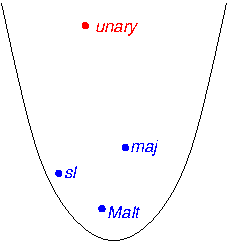
\includegraphics{dichotomy1}}
    \onslide<3|handout:0> \centering{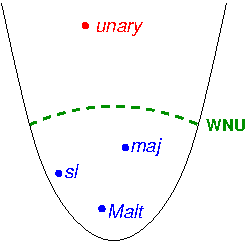
\includegraphics{dichotomy2}}
    \onslide<4|handout:0> \centering{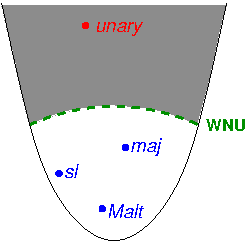
\includegraphics{dichotomy3}}
    \onslide<5-|handout:1>
    \begin{exampleblock}{Supporting Examples}
      \begin{itemize}
      \item Every semilattice and majority op is a WNU.
        
        % \medskip
        %\pause 
      \item<6-> Let \A\ be an abelian group, $n=|A|$. Choose
        integers $k, l$ with $kl \equiv 1 \pmod n$. Then
        \begin{equation*}
          f(x_1,\dots,x_k) = l(x_1+\cdots + x_k)
        \end{equation*}
        is a WNU operation.
      \end{itemize}
    \end{exampleblock}
  \end{overprint}
\end{frame}

\begin{frame}
  \frametitle{Binary Operations}
  A binary operation is  WNU if and only if
  \begin{equation*}
    x\.x = x,\quad x\.y = y\.x.
  \end{equation*}

\pause
  \begin{problem}
    Assume $\Delta$ is a core and $\Pol(\Delta)$
    contains a commutative, idempotent binary operation. Show
    $\CSP(\Delta)$ is tractable.
  \end{problem}

  Recall that a semilattice is an associative WNU.

  \pause
  Note that neither idempotence nor commutativity are sufficient
  individually  
\end{frame}

\begin{frame}
  A left-zero semigroup (i.e., $x\.y=x$) is idempotent, but not
  commutative. It clearly has no WNU.

  \bigpause
  Let $\A=\<\{0,1,2,3\}, \cdot\>$ with multiplication modulo~4. This
  operation is commutative but not idempotent. $\A$ has no WNU.
\end{frame}


\begin{frame}
  Note that \textbf{``has a WNU polymorphism''} puts no bound on the
  number of variables. Is this even decidable?

  \pause
  \begin{theorem}[Siggers, Kearnes, Markovi\'c, McKenzie, 2008
    \cite{Siggers2010,KearnesMarkovicMcKenzieU1}] 
    $\Pol(\Delta)$ has a WNU  if and only if it has a 4-ary idempotent
    operation satisfying
    \begin{equation*}
      t(x,y,z,x) = t(y,z,x,z).
    \end{equation*}
  \end{theorem}

\end{frame}

\bibliographystyle{amsplain} 
\bibliography{amsabbrevs,cliff,univalg,csp}

\end{document}





%%% Local Variables: 
%%% mode: latex
%%% TeX-master: t
%%% End: 
